% REVISÃO DE LITERATURA--------------------------------------------------------

\chapter{REVISÃO TEÓRICA}
\label{chap:fundamentacaoTeorica}

Este capítulo aborda alguns conceitos dos principais componentes e ferramentas utilizadas no projeto.

\section{PROJETO ARQUITETÔNICO}
\label{sec:matrizLed}

O projeto arquitetônico definiu a quantidade, o tipo e a disposição de cada objeto. Ao todo, são 128 sensores reflexivos (infravermelho) e 129 \emph{LEDs RGB}, dispostos sob um tampo acrílico de 1m de diâmetro, conforme apresentado na \autoref{fig:tampo}.

\begin{figure}[H]
    \centering
    \caption{Disposição dos objetos}
    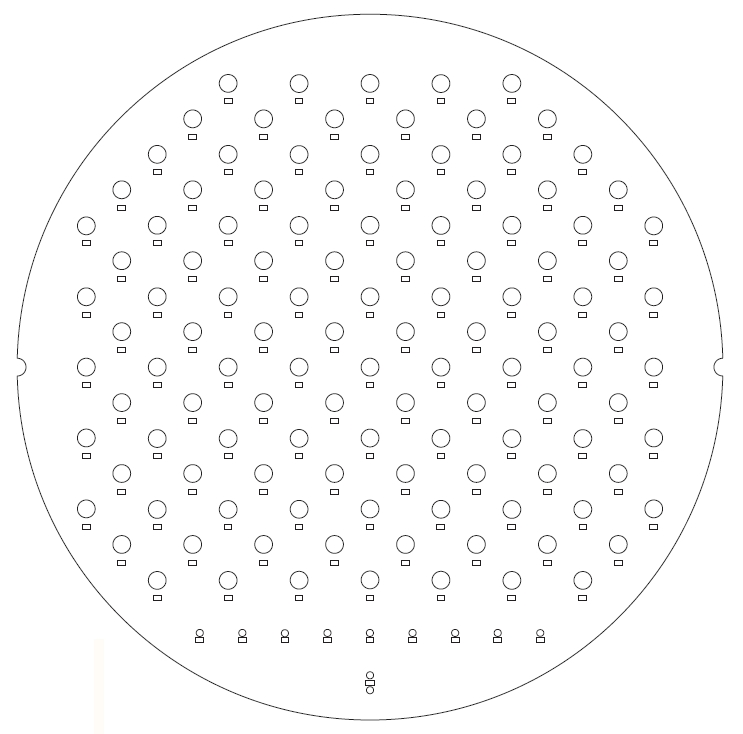
\includegraphics[width=0.8\textwidth]{./dados/figuras/tampo}
    \fonte{MITSUKO, 2016}
    \label{fig:tampo}
\end{figure}

A arquiteta também especifica que o funcionamento da mesa deve ser orientado a eventos, provenientes das seções Controle e Matriz (\autoref{fig:mesa-sup}):

\begin{itemize}[noitemsep]
    \item A mesa sai do modo ocioso ao manter-se a mão sobre a bolinha \emph{Power} por mais de 1s: acende-se o seletor de cores; e a mesa passa a interpretar os demais comandos;
    \item Escolhe-se uma cor ao manter-se a mão sobre uma determinada bolinha do seletor de cores por mais de 1s;
    \item Ao passar a mão sobre uma determinada bolinha da seção Matriz, a mesma deve responder com a última cor escolhida;
    \item Uma bolinha da seção Matriz pode ser apagada se a ``cor'' escolhida tiver sido a da bolinha \emph{Power};
    \item Ao manter-se a mão por mais de 3s sobre a bolinha \emph{Power}, todas as bolinhas da seção Matriz devem ser apagadas; e
    \item Ao manter-se a mão por mais de 5s sobre a bolinha \emph{Power}, a mesa entra em modo ocioso: as bolinhas do seletor de cores são apagadas e a mesa passa a ignorar os comandos sobre a Matriz.
\end{itemize}

A partir da especificação acerca do funcionamento, notam-se alguns desafios do ponto de vista do eletrônico/lógico, tais como:

\begin{itemize}
    \item A disposição dos objetos e o tamanho da mesa;
    \item A capacidade de comandar individualmente 129 \emph{LEDs RGB}, ou seja $129 \times 3 = 387$ canais de cor;
    \item A capacidade de interpretar os níveis lógicos dos 128 sensores;
    \item A capacidade de responder, simultaneamente, aos comandos temporais provenientes de cada sensor.
\end{itemize}

A seleção dos componentes e das ferramentas foi baseada na especificação e nos desafios acima citados, e será discutida a seguir nas demais seções deste capítulo.

\section{SENSOR}
\label{sec:sensor}

A função do sensor é identificar a posição de um objeto, no caso, a mão do espectador, sobre o tampo acrílico, e para manter-se centrado nos objetivos do projeto arquitetônico, a definição do tipo de sensor foi baseada em dois pontos essenciais:

\begin{enumerate}[label=\Roman*.]
    \item O elemento principal do projeto é a luz que flui da bolinha de \emph{ping-pong};
    \item A exposição pode ser levada a diversos lugares e ser instalada nos mais variados ambientes, como museus, escolas, saguões e etc.
\end{enumerate}

A questão (I) implica que o sensor não deve irradiar ondas eletromagnéticas dentro do espectro visível, que vai de $400nm$ a $700nm$ \cite{fundafisica}. Já a questão (II) implica que a instalação será submetida a locais com diferentes graus de iluminação, portanto os sensores devem ser imunes à variação luminosa do ambiente.

Assim sendo, optou-se pelo sensor óptico reflexivo com saída transistorizada \emph{TCRT5000L}, apresentado na \autoref{fig:sensor} e \autoref{fig:sensorop}, cujas características relevantes para o projeto são apresentadas na \autoref{tab:sensor}.

\begin{figure}[!htb]
    \centering
    \caption{Sensor \emph{TCRT5000}}
    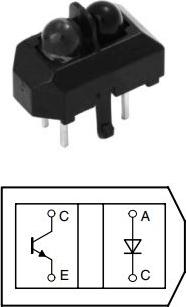
\includegraphics[width=0.2\textwidth]{./dados/figuras/sensor}
    \fonte{\citeonline{datasheetsensor}}
    \label{fig:sensor}
\end{figure}

\begin{figure}[!htb]
    \centering
    \caption{Distância de operação do sensor \emph{TCRT5000}}
    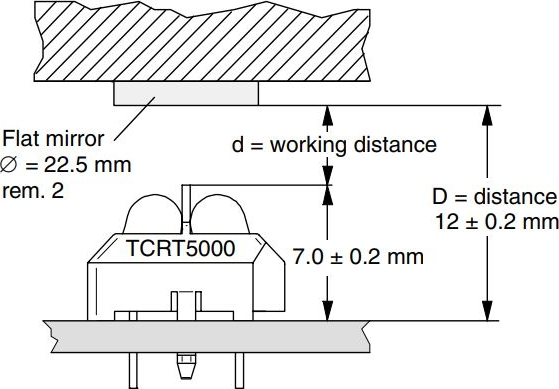
\includegraphics[width=0.45\textwidth]{./dados/figuras/sensor-op}
    \fonte{\citeonline{datasheetsensor}}
    \label{fig:sensorop}
\end{figure}

\begin{table}[H]
    \centering
    \caption[Principais características do sensor]{Principais características do sensor.
    \label{tab:sensor}}
    \begin{tabular}{|l|l|l|l|l|l|l|}
        \hline
        \textbf{Parâmetro} & \textbf{Condição} & \textbf{Símb.} & \textbf{Mín.} & \textbf{Típ.} & \textbf{Máx.} & \textbf{Unidade} \\     \hline
        \emph{LED} - Corrente direta &  & $I_{F}$ &  & 60 &  & mA \\ \hline
        \emph{LED} - Queda direta de tensão & $I_{F} = 60mA$ & $V_{F}$ &  & 1,25 & 1,5 & V \\ \hline
        \emph{LED} - Comprimento de onda & $I_{F} = 100mA$ & $\lambda_{P}$ & 940 &  &  & nm \\ \hline
        Sensor - Corrente de coletor & \begin{tabular}[c]{@{}l@{}}$@5V$,\\ $I_{F} = 10mA$,\\ $D=12mm$\end{tabular} & $I_{C}$ & 0,5 & 1 & 2,1 & mA \\ \hline
        \begin{tabular}[c]{@{}l@{}}Sensor - Queda de tensão entre\\ coletor-emissor na saturação\end{tabular} & \begin{tabular}[c]{@{}l@{}}$I_{F} = 10mA$, \\ $I_{C}=0,1mA$,\\ $D=12mm$\end{tabular} & $V_{CE_{sat}}$ &  &  & 0,4 & V \\ \hline
    \end{tabular}
    \fonte{\citeonline{datasheet-sensor}}
\end{table}


\section{LED}
\label{sec:led}
Protocolo

\section{REGISTRADORES DE DESLOCAMENTO}
\label{sec:registradores}
Falar sobre a IC

\section{MICROCONTROLADOR}
\label{sec:microcontrolador}

\section{\emph{FRAMEWORK}}
\label{sec:framework}

